% ============================================================================
\section{DC-Link Dynamics, Stability, and Voltage Balancing}
\label{sec:dclink_balancing}
% ============================================================================

The shared dc current and independently controllable winding-group
powers (Section~\ref{sec:operating_principle}) make the local
capacitors coupled energy-storage states whose voltages are not
guaranteed to remain equal
\cite{Nikouie2015Stability,Nikouie2017Stability}, a conclusion also
reached independently for a series-connected multilevel motor drive,
where distributed closed-loop current control alone was shown to leave
the module voltages inherently unstable without dedicated balancing
action \cite{Wang2015ThesisDVB}.

For cell $k$,
\begin{equation}
C_kV_{\mathrm{dc},k}\frac{dV_{\mathrm{dc},k}}{dt}
=
V_{\mathrm{dc},k}i_{\mathrm{dc}}
-p_{\mathrm{ac},k}
-p_{\mathrm{loss},k}.
\label{eq:spb_voltage_dynamic}
\end{equation}
This captures the essential balancing mechanism: dc input power
depends directly on local cell voltage because the series current is
common, while output power is set independently by the corresponding
winding group's controller.

For analysis, define
\begin{equation}
\widetilde V_k=
V_{\mathrm{dc},k}
-\frac{1}{N}\sum_{j=1}^{N}V_{\mathrm{dc},j}.
\label{eq:cell_voltage_deviation}
\end{equation}
A simplified differential-mode model around a balanced point is
\begin{equation}
CV_0\frac{d\widetilde V_k}{dt}
\approx
I_{\mathrm{dc},0}\widetilde V_k-\Delta P_k.
\label{eq:linearized_balance_dynamic}
\end{equation}
In motoring operation ($I_{\mathrm{dc},0}>0$), a positive cell-voltage
perturbation increases that cell's dc input power and can reinforce the
deviation if the ac-side power is unchanged; in regeneration the
feedback sign reverses. This simplified picture is consistent with the
detailed SPB stability analyses in
\cite{Nikouie2015Stability,Nikouie2017Stability} and with recent work
on related series-connected multiphase drives
\cite{Ni2025SeriesDCLinkStability}.

Reference~\cite{Nikouie2017Stability} derives this instability directly
from the full nonlinear constant-power-load model, without the
small-signal approximation of \eqref{eq:linearized_balance_dynamic}:
with $L_b\,di_{\mathrm{dc}}/dt=E_b-R_bi_{\mathrm{dc}}-\sum_kV_{\mathrm{dc},k}$
and $C_k\,dV_{\mathrm{dc},k}/dt=i_{\mathrm{dc}}-P_k/V_{\mathrm{dc},k}$, the
open-loop characteristic polynomial has $N-1$ real, strictly positive
eigenvalues in motoring operation ($P_k>0$) for any $N>1$ -- the series
stack is provably unstable without a balancing controller, regardless
of parameter choice. Fig.~\ref{fig:spb_balancing_dynamics} integrates
this exact nonlinear model using the real experimental parameters of
\cite{Nikouie2017Stability} ($L_b=8\,\mu\text{H}$, $R_b=0.35\,\Omega$,
$C=100\,\mu\text{F}$ per cell): without balancing, a small initial
imbalance collapses one cell's voltage within milliseconds, while the
proportional balancing law of \cite{Nikouie2017Stability} (their
``controller alternative I'') drives the same imbalance back to zero on
a comparable timescale.

\begin{figure}[!t]
\centering
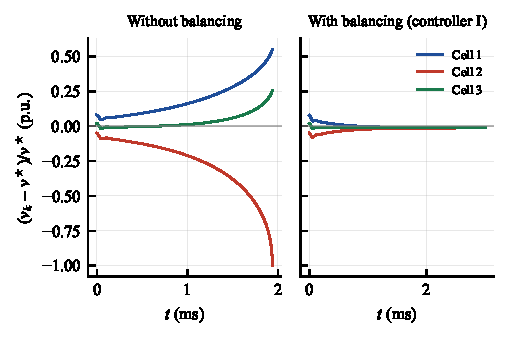
\includegraphics[width=\columnwidth]{Figures/fig_dclink_balancing.pdf}
\caption{Nonlinear dc-link voltage-sharing simulation for $N=3$ cells,
without (left) and with (right) the balancing controller of
\cite{Nikouie2017Stability}. Computed simulation result, not measured
hardware data.}
\label{fig:spb_balancing_dynamics}
\end{figure}

The multiple winding groups provide a natural actuator for controlling
internal capacitor energy. The cell power reference can be decomposed
as
\begin{equation}
P_k^\star=\frac{P^\star}{N}+\Delta P_k,
\qquad
\sum_{k=1}^{N}\Delta P_k=0,
\label{eq:balancing_power}
\end{equation}
so differential power redistributes internal energy without changing
the requested total machine power. In practice $\Delta P_k$ is limited
by phase-current margin, winding voltage, torque-ripple constraints,
and thermal state, so balancing authority is operating-point
dependent.

Three main SPB balancing approaches can be identified. Centralized
active balancing uses measured capacitor voltages to generate
differential current or power commands
\cite{Nikouie2015Stability,Nikouie2017Stability}. Common-duty-ratio
(CDR) control applies common modulation commands and can obtain stable
voltage sharing from the natural converter--machine dynamics for the
investigated induction-machine system \cite{Mocevic2023CDR}, though
practical timing mismatch remains important
\cite{Mocevic2024GateDelay}. Distributed multi-agent control uses local
measurements and neighbour communication, and has been demonstrated
for voltage balancing, power sharing, and reconfiguration
\cite{Verkroost2024VoltageBalance,Verkroost2024PowerDistribution,
Verkroost2024Reconfiguration}, comparable to the local droop laws that
coordinate power sharing across modules in the speed-droop framework of
Galassini \textit{et al.} \cite{Galassini2016ModularSpeedDroop}.
Table~\ref{fig:spb_balancing_taxonomy} summarizes these approaches and
their principal considerations.

\begin{table}[!t]
\centering
\caption{Principal SPB dc-link balancing approaches and their main
considerations.}
\label{fig:spb_balancing_taxonomy}
\renewcommand{\arraystretch}{1.15}
\setlength{\tabcolsep}{3pt}
\footnotesize
\begin{tabular}{p{1.6cm}p{2.9cm}p{2.6cm}}
\hline
\textbf{Approach} & \textbf{Mechanism} & \textbf{Key consideration}\\
\hline
Centralized & Differential current/power commands
\cite{Nikouie2015Stability,Nikouie2017Stability} &
Direct authority; global sensing and coordination\\
CDR & Common modulation, natural coupled dynamics
\cite{Mocevic2023CDR,Mocevic2024GateDelay} &
Low overhead; symmetry- and timing-sensitive\\
Distributed & Local agents, neighbour communication
\cite{Verkroost2024VoltageBalance,Verkroost2024PowerDistribution,
Verkroost2024Reconfiguration} &
Scalable; requires communication and synchronization\\
\hline
\end{tabular}
\end{table}

For automotive operation, balancing must remain effective through
torque transients, field weakening, parameter mismatch, and module
reconfiguration: voltage-sensor offset, communication latency,
propagation delay, and the available differential current/power margin
can determine the usable cell-voltage margin and, consequently, the
semiconductor rating.

This underscores the section's central point: dc-link stability
belongs to the complete converter--machine--control system, not the
power stage alone.
